%%%%%%%%%%%%%%%%%%%%%%%%%%%%%%%%%%%%%%%%%%%%%%%%%%%%%%
% A Beamer template for Ritsumeikan University       %
% Author: Ming-Hao Xu (Xu Minghao)                   %
% Date:   April 2022.                                %
% LPPL Licensed.                                     %
%%%%%%%%%%%%%%%%%%%%%%%%%%%%%%%%%%%%%%%%%%%%%%%%%%%%%%

% ------------------------------ Document format details --------------------------------------

\documentclass{beamer}
\usepackage{hyperref}
% \usepackage[T1]{fontenc}
\usefonttheme{serif}

% other packages
\usepackage{latexsym,amsmath,multicol,booktabs,calligra}
\usepackage{pstricks,listings,stackengine}
% dummy text; remove it when working on this template
\usepackage{lipsum}
% \usepackage[table,xcdraw,svgnames]{xcolor}  % or
% \usepackage[usenames,dvipsnames,svgnames,table]{xcolor}  % more named colors
% \usepackage[html]{xcolor}  % For direct hex use
\usepackage[table,svgnames,dvipsnames]{xcolor}
% \usepackage[table]{xcolor}
\usepackage{graphicx}
\usepackage{subcaption}

% \usepackage{xcolor}
\usepackage{tikz}

\usepackage{booktabs}
\usepackage{subcaption}
\usepackage{lmodern}
% \usepackage[margin=1in]{geometry}
% \usepackage{enumitem}
% \definecolor{googleBlue}{HTML}{4285F4}
% \definecolor{googleGreen}{HTML}{34A853}
% \definecolor{googleYellow}{HTML}{FBBC05}
% \definecolor{googleRed}{HTML}{EA4335}


% --------------------------------- Title page edits ------------------------------------------

% Cointegration shared = Cointegrated time series with a common cointegrating vector
% Cointegration correlated = Spurious correlation

\author[Big4]{\large \textsc{Big 4}\\
\scriptsize \textbf{\textit{Ramakrishna Mission Vivekananda \\Educational and Research Institute Belur}}}
\title[Cointegration]{Cointegration\\\small Uncovering long-run relationships in time series}

\institute[RKMVERI Belur]{
    \textbf{Team Members}\\
    \texttt{Banerjee Ayan, Bhattacharya Darpan, \\Bhattacharya Soham, Bodhak Soham}
}
\date{\today}
\usepackage{Ritsumeikan}
% \usethem

% ----------------------------------------- defs ---------------------------------------------
\def\cmd#1{\texttt{\color{red}\footnotesize $\backslash$#1}}
\def\env#1{\texttt{\color{blue}\footnotesize #1}}
\definecolor{deepblue}{rgb}{0,0,0.5}
\definecolor{deepred}{rgb}{0.6,0,0}
\definecolor{deepgreen}{rgb}{0,0.5,0}
\definecolor{halfgray}{gray}{0.55}

\lstset{
    basicstyle=\ttfamily\small,
    keywordstyle=\bfseries\color{deepblue},
    emphstyle=\ttfamily\color{deepred},    % Custom highlighting style
    stringstyle=\color{deepgreen},
    numbers=left,
    numberstyle=\small\color{halfgray},
    rulesepcolor=\color{red!20!green!20!blue!20},
    frame=shadowbox,
}

% ------------------------------------ Document Begins ----------------------------------------

\begin{document}

\begin{frame}
    \titlepage
    \begin{figure}[htpb]
        \centering
        
\includegraphics[width=0.05\linewidth]{images/logo.png}
    \end{figure}
\end{frame}

\begin{frame}
    \tableofcontents[sectionstyle=show,subsectionstyle=show/shaded/hide,subsubsectionstyle=show/shaded/hide]
\end{frame}


% ---------------------- Content -----------------------
% \section{Timeline}
% "Cointegration shared" ≈ long-term equilibrium
% "Cointegration correlated" ≈ Correlation in short-term behavior ≈ short-term dynamics

\begin{frame}{Timeline}
	\begin{center}
		\begin{tikzpicture}
			% Timeline line
			\draw[thick] (0,0) -- (8,0);
			
			% Events
			\foreach \x/\year/\label in {0/\small Week 1/\small Kickoff, 2/\small Week 2/\small Stationarity, 4/\small Week 3/\small Johansen, 6/\small Week 4/\small ECM, 8/\small Week 5/\small Wrap-up} {
				\draw[fill=ritsumeikan] (\x,0) circle (4pt);
				\node[above] at (\x,0.2) {\textbf{\year}};
				\node[below] at (\x,-0.2) {\label};
			}
		\end{tikzpicture}
	\end{center}
\end{frame}

\begin{frame}{Week 1}
	\textbf{Period: }(Oct 7 – Oct 13)
	\begin{itemize}
		\item Team discussion \& work distribution (who handles dataset search, coding, slides, etc.).
		\item Finalize dataset (e.g., macroeconomic/financial variables).
		\item Everyone revises basics: stationarity, ADF/PP tests, cointegration concept.
	\end{itemize}
\end{frame}

\begin{frame}{Week 2}
	\textbf{Period: }(Oct 14 – Oct 20)
	\begin{itemize}
		\item Perform unit root tests (ADF/PP) on chosen variables.
		\item Share results among team \& discuss division of analysis.
		\item Start applying Engle–Granger 2-step test for initial cointegration check.
	\end{itemize}
\end{frame}

\begin{frame}{Week 3}
	\textbf{Period: }(Oct 21 – Oct 27)
	\begin{itemize}
		\item Run Johansen cointegration test for multiple series.
		\item Identify cointegrating vectors \& interpret results.
		\item Team sync-up: assign one subgroup to results interpretation and one to visuals/plots.
	\end{itemize}
\end{frame}

\begin{frame}{Week 4}
	\textbf{Period: }(Oct 28 – Nov 3)
	\begin{itemize}
		\item Develop Error Correction Model (ECM) to show short-run vs long-run dynamics.
		\item Validate with diagnostic checks and finalize output tables/graphs.
		\item Start making presentation slides (intro, methodology, results, discussion).
	\end{itemize}
\end{frame}

\begin{frame}{Week 5}
	\textbf{Period: }(Nov 4 – Nov 7)
	\begin{itemize}
		\item Team discussion \& rehearsal: combine slides from all members.
		\item Final check: clarity, timing, flow of presentation.
		\item Submit final slides/report if required.
		\item Practice dry run before presentation day.
	\end{itemize}
\end{frame}

\section{Pre-requisites}

\begin{frame}{Prerequisites}
	\begin{center}
		\Huge
		Time Series
	\end{center}
\end{frame}
	
\begin{frame}[allowframebreaks]
	\frametitle{Examples}
	\begin{figure}[H]
		\centering
		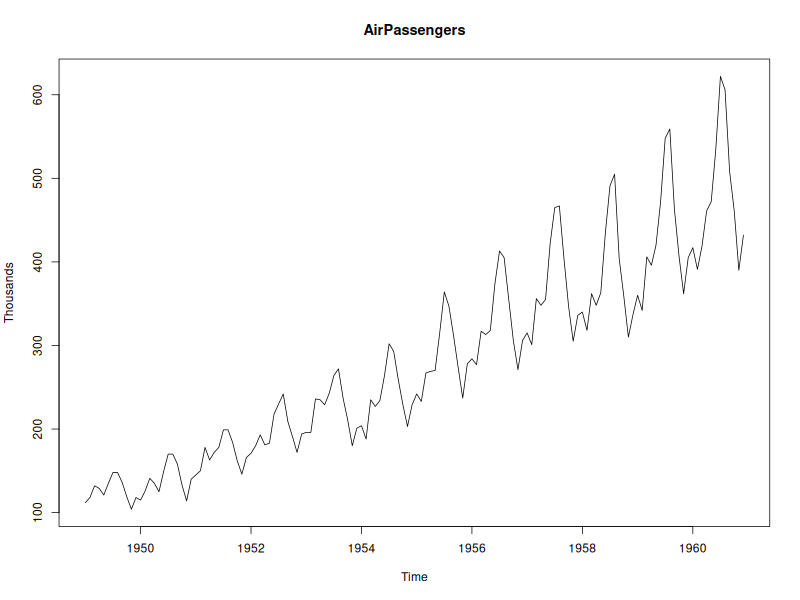
\includegraphics[width=0.75\linewidth]{images/AirPassengers__plot.png}
		\caption{Example of a \textbf{non-stationary} time series}
	\end{figure}
	\small
	Refer: Monthly airline passengers (1949-1960) [R-datasets]
	
	\framebreak
	
	\begin{figure}[H]
		\centering
		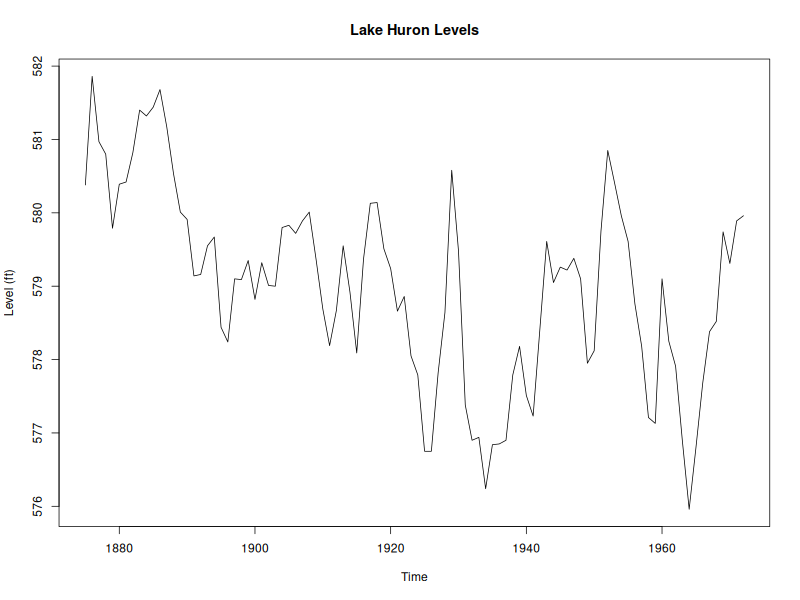
\includegraphics[width=0.75\linewidth]{images/LakeHuron_plot.png}
		\caption{Example of a \textbf{nearly stationary} time series}
	\end{figure}
	\small
	Refer: Annual level of Lake Huron (1875-1972) [R-datasets]
	
	\framebreak
	
	\begin{figure}[H]
		\centering
		
\includegraphics[width=0.75\linewidth]{notes/stationary_ts.png}
		\caption{Example of a \textbf{stationary} time series}
	\end{figure}
	\small
	It is AR(1) process.
	
	\framebreak
\end{frame}

\begin{frame}[allowframebreaks]
	\frametitle{Pre-requisites}
	\textbf{What is a stationary time series?}
	
	A stationary time series is one whose statistical properties do not change over time. Formally, a time series {$y_t$} is weakly stationary if:
	\begin{itemize}
		\item Constant mean: E[$y_t$] = $\mu$ $\forall\ t$
		\item E[$y_t^2$] $< \infty$
		\item Covariance depends only on lag: Cov($y_t, y_{t-k}$) = $\gamma_k$, which only depends on the lag $k$ and not on time $t$.
	\end{itemize}
	
	\framebreak
	
	\textbf{Unit root geometrically}
	
	\begin{itemize}
		\item A unit root means one of these roots lie on the unit circle, i.e., $|z|=1$. Eg: $y_t = \phi y_{t-1} + a_t$.
		
		\item Characteristic equation: $1 - \phi B = 0 \implies B = \frac{1}{\phi}$.
		
		\begin{itemize}
			\item If $|\phi|<1$, then the root lies outside the unit circle $\implies$ stationary.
			
			\item If $|\phi|=1$, then the root lies exactly on the unit circle $\implies$ unit root non-stationary.
			
			\item If $|\phi|>1$, then the root lies outside the unit circle $\implies$ explosive series.
		\end{itemize}
	\end{itemize}
	
	\framebreak
	
	\begin{table}[h!]
		\centering
		\tiny
		\begin{tabular}{llll}
			\toprule
			\textbf{Property} & \textbf{Stationary} & \textbf{Unit Root} & \textbf{Differenced} \\
			& & \textbf{(Nonstationary)} & \textbf{(Stationary)}\\
			
			\midrule
			Equation & $y_t = 0.5y_{t-1} + a_t$ & $y_t = y_{t-1} + a_t$ & $\Delta y_t = a_t$ \\
			
			Process Type & AR(1), $I(0)$ & Random Walk, $I(1)$ & White Noise, $I(0)$ \\
			
			Stationarity & Yes & No & Yes \\
			\bottomrule
		\end{tabular}
		\caption{Comparison of stationary, unit root, and differenced time series.}
		\label{tab:ts_comparison}
	\end{table}
\end{frame}

%\section{Introduction}
%\section{Why cointegration?}
\section{Why?}
% "Cointegration shared" ≈ long-term equilibrium
% "Cointegration correlated" ≈ Correlation in short-term behavior ≈ short-term dynamics

%How We Test for Unit RootsGoal: Before we can model our data, we must check if it's $I(0)$ or $I(1)$.The Test: We use a Unit-Root Test, such as the Augmented Dickey-Fuller (ADF) Test (Section 5.1.6).How it Works: The ADF test runs a regression like:$\Delta z_t = \beta z_{t-1} + \sum \phi_i^* \Delta z_{t-i} + a_t$Hypotheses:Null ($H_0$): $\beta = 0$ $\rightarrow$ The series has a unit root (it is $I(1)$).Alternative ($H_a$): $\beta < 0$ $\rightarrow$ The series is stationary (it is $I(0)$).Action: "For our project, we will first run the ADF test on all our variables. We expect to fail to reject the null, proving they are $I(1)$."

\begin{frame}{Problem}
	\textbf{How do we test for unit roots?}
	Goal?
\end{frame}

\begin{frame}[allowframebreaks]
	\frametitle{Unit roots testing}
	
	\textbf{Aim}: Check if the data is $I(0)$ or $I(1)$.
	
	\textbf{Test}: Augmented Dickey-Fuller (ADF) test
	
	\textbf{Method}: Run the following regression:
	$$\Delta z_t = \beta z_{t-1} + \sum \phi_i^* \Delta z_{t-i} + a_t$$
	
	\framebreak
	
	\textbf{Hypothesis testing}
	\begin{itemize}
		\item $H_0: \beta = 0 \rightarrow \exists$ a unit root ($I(1)$)
		\item $H_1: \beta < 0 \rightarrow$ stationary ($I(0)$)
	\end{itemize}
\end{frame}


\subsection{Problem}
\begin{frame}{Problem}
	%\textbf{Problem}
	\begin{center}
		Most real-world data are non-stationary.
	\end{center}
\end{frame}

\subsection{Trap}
\begin{frame}[allowframebreaks]
	\frametitle{The trap}
	
	\begin{figure}[H]
		\centering
		
\includegraphics[width=\linewidth]{notes/twoRwalks.png}
		\caption{Two random walks}
	\end{figure}
	\framebreak
	
	%A \textbf{spurious regression} happens when you regress one non-stationary time series on another non-stationary time series that is not actually related.
	
	\begin{itemize}
		\item A \textbf{regression} may show a high R² and significant t-statistics, even though there is no real relationship between the variables.
		\item The regression is `\textbf{spurious}' or `\textbf{fake}'. It captures the common trends, not a true economic relationship. This is a major pitfall.
	\end{itemize}
	\framebreak
	
	\textbf{Example}:
	\small
	
	Suppose
	\begin{itemize}
		\item $X_t$ = global temperature over time
		\item $Y_t$ = stock prices over time
	\end{itemize}
	Both may increase over decades, so a regression explaining the phenomena would be:
	$$Y_t = \alpha + \beta X_t + \epsilon_t$$
	might show a very high $R^2$ and a significant $\beta$ due to its shared trend, not because of the variables affecting each other. But \texttt{temperatures} \& \texttt{stock prices} do not affect each other in real-world scenario. Hence this type of regression is called \textbf{spurious regression}.
\end{frame}

\begin{frame}[allowframebreaks]
	\frametitle{Correlation vs Cointegration}
	\begin{table}[h!]
		\centering
		\tiny
		\begin{tabular}{lll}
			\toprule
			
			\textbf{Feature} & \textbf{Correlation} & \textbf{Cointegration} \\ 
			
			\midrule
			
			\textbf{Time frame} & Short-term link & Long-term link \\ 
			
			\textbf{Type of data} & Works with any data & Needs non-stationary series \\ 
			
			\textbf{Focus} & Linear co-movement & Long-run equilibrium \\ 
			
			\textbf{Nature} & Simple dependence & Complex, involves stationarity \\ 
			
			\textbf{Example} & Two stocks move together & Oil and gas prices linked \\ 
			
			\bottomrule
		\end{tabular}
		\caption{Correlation vs. Cointegration comparison}
		\label{tab:corr__coint}
	\end{table}
\end{frame}

%\begin{frame}{Summary}
%	\begin{itemize}
%		\item \textbf{Correlation}: It is concerned with how two variables move together, but it is usually a \textit{short-term} or \textit{momentary measure}.
		
%		\item \textbf{Cointegration}: Deals with the long-term equilibrium between two non-stationary variables, implying that they share a common trend and are bound together in the long run.
%	\end{itemize}
%\end{frame}
%\section{Cointegration}
%\section{What is cointegration?}
\section{What?}

\subsection{Definition}
\begin{frame}[allowframebreaks]
	\frametitle{Co-integration}
	\centering
	What is \textbf{Co-integration}?
	\framebreak
	
	\textbf{Definition}: Two time series $X_t$, $Y_t$ are cointegrated if:
	\begin{itemize}
		\item Each series is \textbf{integrated of order 1} [\textit{I(1)}] $\rightarrow$ they become stationary after first differencing.
		\item $\exists$ a linear combination, say $u_t = Y_t$ - $\beta X_t$, which becomes \textbf{stationary [I(0)]}.
	\end{itemize}
	\framebreak
	
	\begin{itemize}
		\item A vector of \texttt{k} time series is said to be \textbf{cointegrated} if \textit{individual components are non-stationary} but $\exists$ a linear combination $\beta$ such that $w_t = \beta'z_t$ is \textit{stationary}.
		
		\item If there are \texttt{m} such vectors linearly independent, it means that $\exists$ \texttt{m} cointegrating relationships and \texttt{k-m} sources of non-stationarity.
	\end{itemize}
	\framebreak
	
	\textbf{Examples}
	\begin{itemize}
		\item Purchasing power parity.
		\item Pair trading in stock market.
		\item Income and consumption.
	\end{itemize}
\end{frame}

\begin{frame}{Role of cointegration}
	Cointegration is about long-run equilibrium relationships between non-stationary I(1) variables.
	
	\begin{itemize}
		\item If two or more series share a \textit{common stochastic trend}, then some \textbf{linear combination} of them will be \textbf{stationary I(0)}.
		$$y_t \sim I(1),\ x_t \sim I(1)\ but\ (y_t - \beta x_t) \sim I(0)$$
		
		\item Cointegration does not depend on whether each individual time series is AR, MA or ARMA. Their order of integration matters.
	\end{itemize}
\end{frame}


\subsection{Example}

\begin{frame}[allowframebreaks]
	\frametitle{Example}
	
	Consider a \textbf{bivariate (k=2) VARMA(1,1)}
	
	$$
	\begin{bmatrix} z_{1t} \\ z_{2t} \end{bmatrix} -
	\begin{bmatrix} 0.5 & -1.0 \\ -0.25 & 0.5 \end{bmatrix}
	\begin{bmatrix} z_{1,t-1} \\ z_{2,t-1} \end{bmatrix} =
	\begin{bmatrix} a_{1t} \\ a_{2t} \end{bmatrix} -
	\begin{bmatrix} 0.2 & -0.4 \\ -0.1 & 0.2 \end{bmatrix}
	\begin{bmatrix} a_{1,t-1} \\ a_{2,t-1} \end{bmatrix}$$
	
	This is in the form $\Phi(B)z_t = \Theta(B)a_t$, where $\Phi(B)$ is the AR coefficient matrix \& $\Theta(B)$ is the white noise coefficient matrix.
	
	\framebreak
	
	\textbf{The system is nonstationary}
	
	\textbf{Observations}
	\begin{itemize}
		\item The AR coefficient matrix $\Phi$ has eigenvalues of 0 and 1. 
		\item The eigenvalue of 1 causes non-stationarity.
		\item The eigenvectors are (1.0, -2.0)$^t$ \& (0.5, 1.0)$^t$ corresponding to the eigenvalues 0 \& 1 respectively.
	\end{itemize}
	
	\framebreak
	
	We apply a special transformation matrix $L$ to create a new system 
	
	$y_t$:$$\begin{bmatrix} y_{1t} \\ y_{2t} \end{bmatrix} =
	\begin{bmatrix} 1.0 & -2.0 \\ 0.5 & 1.0 \end{bmatrix}
	\begin{bmatrix} z_{1t} \\ z_{2t} \end{bmatrix} \quad \text{or} \quad y_t = Lz_t$$
	
	\framebreak
	
	So, L = $$\begin{bmatrix} 1.0 & -2.0 \\ 0.5 & 1.0 \end{bmatrix}$$ and let $y_t = Lz_t$.
	
	So,
	$$y_{1t} = 1.0 z_{1t} - 2.0 z_{2t}$$
	$$y_{2t} = 0.5 z_{1t} + 1.0 z_{2t}$$
	
	\begin{itemize}
		\item $y_{1t} \implies$ common trend due to I(1) non-stationarity.
		\item $y_{2t} \implies$ white noise due to I(0) stationarity.
	\end{itemize}
	
	%The $\Pi$ matrix is singular: As we learned, $\Pi = -\Phi(1) = -(I - \Phi_1)$. The text states $|\Phi(1)| [cite_start]= 0$, which confirms the system has a unit root and is nonstationary4.
	
	%\framebreak
	
	%Now, proving the Individual Series are $I(1)$.
	
	%Through algebraic manipulation, we get
	
	%$$\begin{bmatrix} 1-B & 0 \\ 0 & 1-B \end{bmatrix}
	%\begin{bmatrix} z_{1t} \\ z_{2t} \end{bmatrix} =
	%\begin{bmatrix} 1-0.7B & -0.6B \\ -0.15B & 1-0.7B \end{bmatrix}
	%\begin{bmatrix} a_{1t} \\ a_{2t} \end{bmatrix}$$This equation shows that $(1-B)z_t = \Delta z_t$ is a stationary VMA(1) process.
	
	%Interpretation: Because you have to difference $z_{1t}$ and $z_{2t}$ to make them stationary, this proves that both $z_{1t}$ and $z_{2t}$ are $I(1)$ (unit-root) processes6. This is the setup for a spurious regression: we have two $I(1)$ series.
	
	
	
	%Why this specific matrix? It was specially chosen to "uncover" the hidden structure. When you apply this transformation to the original VARMA(1,1) model, the math simplifies to Equation (5.64):$$\begin{bmatrix} y_{1t} \\ y_{2t} \end{bmatrix} -
	%\begin{bmatrix} 1.0 & 0 \\ 0 & 0 \end{bmatrix}
	%\begin{bmatrix} y_{1,t-1} \\ y_{2,t-1} \end{bmatrix} =
	%\begin{bmatrix} b_{1t} \\ b_{2t} \end{bmatrix} -
	%\begin{bmatrix} 0.4 & 0 \\ 0 & 0 \end{bmatrix}
	%\begin{bmatrix} b_{1,t-1} \\ b_{2,t-1} \end{bmatrix}$$where $b_t = La_t$ is the new white noise term7.Part 4: The Result — Interpreting the New SystemThis new, diagonal system is easy to interpret. Let's look at the equation for each $y_t$ variable separately:Equation for $y_{1t}$:$y_{1t} - 1.0 y_{1,t-1} = b_{1t} - 0.4 b_{1,t-1}$This is a nonstationary ARIMA(0,1,1) model. This series $y_{1t}$ is the common trend that drives both $z_{1t}$ and $z_{2t}$.Equation for $y_{2t}$:$y_{2t} - 0 y_{2,t-1} = b_{2t} - 0 b_{2,t-1}$This simplifies to $y_{2t} = b_{2t}$. Since $b_{2t}$ is just white noise (a linear combination of $a_t$), this equation shows that $y_{2t}$ is stationary ($I(0)$)8.Part 5: The Grand Conclusion — Cointegration!This is the final step that ties it all together:We proved in Part 2 that $z_{1t}$ and $z_{2t}$ are both $I(1)$.We proved in Part 4 that the linear combination $y_{2t} = 0.5 z_{1t} + 1.0 z_{2t}$ is $I(0)$ (stationary).By definition, if a linear combination of $I(1)$ series is $I(0)$, the series are cointegrated.The cointegrating vector (the "leash") is $\beta' = [0.5, 1.0]$9.The common trend (the "person" everyone is following) is $y_{1t} = 1.0 z_{1t} - 2.0 z_{2t}$10.
\end{frame}

\subsection{Method}

\begin{frame}[allowframebreaks]
	\frametitle{Error Correction Model (ECM)}
	\begin{itemize}
		\item \textit{Engle-Granger} suggested the \textbf{ECM form}. This is a different algebraic representation for the same \texttt{VARMA} model that is \textbf{stationary} and \textbf{invertible}.
		
		\item ECM form of a VARMA(p,q) model (VECM itself):
		$$\Delta z_t = \boldsymbol{\Pi} z_{t-1} + \sum_{i=1}^{p-1} \boldsymbol{\Phi_i}^* \Delta z_{t-i} + c(t) + \boldsymbol{\Theta(B)}a_t$$
		
		\item For univariate case, it is simply ECM; for \textit{multivariate} cases, it is \textbf{VECM (Vector Error Correction Model)}
	\end{itemize}
	
	\framebreak
	
	VECM form of VARMA(p,q):
	$$\Delta z_t = \boldsymbol{\Pi} z_{t-1} + \sum_{i=1}^{p-1} \boldsymbol{\Phi_i}^* \Delta z_{t-i} + c(t) + \boldsymbol{\Theta(B)}a_t$$
	
	where 
	\begin{enumerate}
		\item $\sum_{i=1}^{p-1} \boldsymbol{\Phi_i}^* \Delta z_{t-i}$ captures the short-run dynamics.
		
		\item $c(t) + \boldsymbol{\Theta(B)}a_t$ is the stationary part.
		
		\item $\boldsymbol{\Pi} z_{t-1}$ is the error correction term.
	\end{enumerate}
\end{frame}


\begin{frame}[allowframebreaks]
	\frametitle{VECM}
	\small
	For \textbf{VAR(2)} model,
	$$z_t = c_0 + \boldsymbol{\phi}_1 z_{t-1} + \boldsymbol{\phi}_2 z_{t-2} + a_t$$.
	
	To make it stationary, we difference it once,
	$$z_t  - z_{t-1} = c_0 + \boldsymbol{\phi}_1 z_{t-1} - z_{t-1} + \boldsymbol{\phi}_2 z_{t-2} + a_t$$
	
	$$\implies \Delta z_t = c_0 + (\boldsymbol{\phi}_1 - \boldsymbol{I})z_{t-1} + \boldsymbol{\phi}_2 z_{t-2} + a_t$$
	
	$$\implies \Delta z_t = c_0 + \boldsymbol{\Pi} z_{t-1} + \boldsymbol{\Phi}_1^* \Delta z_{t-1} + a_t$$
	where
	$$\boldsymbol{\Pi} = (\boldsymbol{\phi}_1 + \boldsymbol{\phi}_2 - \boldsymbol{I}),\ \boldsymbol{\Phi}_1^* = \boldsymbol{-\phi}_2$$
	
	\framebreak
	
	In general, \textbf{VECM} model looks like
	
	$$\Delta z_t = c(t) + \boldsymbol{\Pi} z_{t-1} + \sum_{i=1}^{p-1} \boldsymbol{\Phi}_i^* \Delta z_{t-i} + a_t$$
	
	where
	
	$$\boldsymbol{\Pi} = -(\boldsymbol{I} - \sum_{i=1}^{p} \boldsymbol{\phi}_i)\ \&\ \boldsymbol{\Phi}_i^* = -(\sum_{j=i+1}^{p}\boldsymbol{\phi}_i)$$
\end{frame}
%\section{How is cointegration tested?}
%\section{Cointegration test}
\section{How?}

\begin{frame}[allowframebreaks]
	\frametitle{Johansen test}
	\small
	\begin{itemize}
		\item \textbf{Goal}: We need a formal test to find out if cointegration exists and, if so, how many (i.e., how many ``leashes").
		
		\item \textbf{Test}: The Johansen test (Section 5.9) is the standard tool.
		
		\item \textbf{The model}: Vector Error-Correction Model (VECM) form (from Section 5.6):
		$$\Delta z_t = \boldsymbol{\Pi} z_{t-1} + \sum_{i=1}^{p-1} \boldsymbol{\Phi_i}^* \Delta z_{t-i} + c(t) + \boldsymbol{\Theta(B)}a_t$$
		
		\item \textbf{Objective}: To check for the rank ($m$) of the $\boldsymbol{\Pi}$ matrix which is the number of cointegrating vectors.
		\begin{itemize}
			\item If $\text{Rank}(\boldsymbol{\Pi}) = 0$, the series are not cointegrated.
			
			\item If $\text{Rank}(\boldsymbol{\Pi}) = m > 0$, there are $m$ cointegrating vectors.
		\end{itemize}
	\end{itemize}
	\framebreak
	
	\begin{itemize}
		\item \textbf{Test statistics}: The test produces two statistics (Section 5.9.4):
		\begin{enumerate}
			\item Trace statistic ($L_{tr}$): Tests 
			$$H_0: \text{Rank} = m\ vs.\ H_a: \text{Rank} > m$$
			
			\item Max-Eigenvalue statistic ($L_{max}$): Tests 
			$$H_0: \text{Rank} = m\ vs.\ H_a: \text{Rank} = m+1$$
		\end{enumerate}
		
		\item $L_{tr}(m) = -(T - kp) \sum_{i=m+1}^{k} \ln(1 - \lambda_i)$
		
		\item $L_{max}(m) = -(T - kp) \ln(1 - \lambda_{m+1})$
		\item We keep testing sequentially for all values of \textit{m} until it reaches Rank($\boldsymbol{\Pi}$).
	\end{itemize}
\end{frame}

\begin{frame}[allowframebreaks]
	\frametitle{Example}
	\small
		
	\textbf{Setup:}
	We have two nonstationary (\(I(1)\)) series \(z_t = (z_{1t}, z_{2t})'\), and we wish to test for the number of cointegrating relationships.
	
	\textbf{Step 1: Set up the ECM Model}
	Choose a VAR order \(p = 2\). Based on the text, the Error-Correction Model (ECM) is:
	\[
	\Delta z_t = c_0 + \boldsymbol{\Pi} z_{t-1} + \boldsymbol{\Phi}_1^* \Delta z_{t-1} + a_t
	\]
	Our goal is to determine the \emph{rank} (\(m\)) of the \(2\times2\) matrix \(\boldsymbol{\Pi}\):
	\begin{itemize}
		\item \(m = 0\): no cointegration,
		\item \(m = 1\): one cointegrating vector,
		\item \(m = 2\): both series are stationary.
	\end{itemize}
	
	\framebreak
	\textbf{Step 2: Run ``Helper'' Regressions}
	We cannot test \(\boldsymbol{\Pi}\) directly. We first concentrate out short-run dynamics:
	\begin{enumerate}
		\item Regress \(\Delta z_t\) on a constant and \(\Delta z_{t-1}\); save residuals \(\hat{u}_t\).
		\item Regress \(z_{t-1}\) on a constant and \(\Delta z_{t-1}\); save residuals \(\hat{v}_t\).
	\end{enumerate}

	\framebreak
	\textbf{Step 3: Compute Covariance Matrices}
	From the residuals, we compute sample covariance matrices (hypothetical values):
	\[
	\hat{\Sigma}_{00} = 
	\begin{bmatrix}
		4 & 1\\
		1 & 3
	\end{bmatrix}, \quad
	\hat{\Sigma}_{11} =
	\begin{bmatrix}
		5 & 2\\
		2 & 2
	\end{bmatrix}, \quad
	\hat{\Sigma}_{01} =
	\begin{bmatrix}
		3 & 1.5\\
		1 & 1
	\end{bmatrix}, \quad
	\hat{\Sigma}_{10} = \hat{\Sigma}_{01}' =
	\begin{bmatrix}
		3 & 1\\
		1.5 & 1
	\end{bmatrix}
	\]
	
	\framebreak
	\textbf{Step 4: Solve the Eigenvalue Problem}
	The Johansen test uses the eigenvalues of
	\[
	S = \hat{\Sigma}_{11}^{-1}\hat{\Sigma}_{10}\hat{\Sigma}_{00}^{-1}\hat{\Sigma}_{01}.
	\]
	
	\framebreak
	\textbf{Calculations:}
	\begin{enumerate}
		\item Find inverses:
		\[
		|\hat{\Sigma}_{00}| = 11, \quad 
		\hat{\Sigma}_{00}^{-1} = \tfrac{1}{11}
		\begin{bmatrix}
			3 & -1\\
			-1 & 4
		\end{bmatrix}, \quad
		|\hat{\Sigma}_{11}| = 6, \quad
		\hat{\Sigma}_{11}^{-1} = \tfrac{1}{6}
		\begin{bmatrix}
			2 & -2\\
			-2 & 5
		\end{bmatrix}
		\]
		\item Multiply to obtain:
		\[
		S =
		\begin{bmatrix}
			0.3636 & 0.1591\\
			0.2273 & 0.1932
		\end{bmatrix}
		\]
		\item Eigenvalues of \(S\):
		\[
		\lambda_1 \approx 0.487, \qquad \lambda_2 \approx 0.070
		\]
	\end{enumerate}
	
	\framebreak
	\textbf{Step 5: Compute Test Statistics}
	
	Effective sample size: \(T - kp = 196\).
	
	\textbf{Trace Statistic:}
	$$L_{\mathrm{tr}}(0) = -196 \left[\ln(1 - 0.487) + \ln(1 - 0.070)\right]$$
	$$= -196[-0.667 - 0.072] \approx \mathbf{144.8}$$
	
	$$L_{\mathrm{tr}}(1) = -196 \ln(1 - 0.070)
	= -196[-0.072] \approx \mathbf{14.1}$$
	
	\textbf{Max-Eigenvalue Statistic:}
	$$L_{\max}(0) = -196 \ln(1 - 0.487)
		= -196[-0.667] \approx \mathbf{130.7}$$
		
	$$L_{\max}(1) = -196 \ln(1 - 0.070)
	= -196[-0.072] \approx \mathbf{14.1}$$
	
	\framebreak
	\textbf{Step 6: Compare with Critical Values}
	\centering
	\renewcommand{\arraystretch}{1.2}
	\begin{tabular}{lcccc}
		\hline
		\textbf{Hypothesis} & \textbf{Statistic} & \textbf{Value} & \textbf{5\% CV} & \textbf{Decision}\\
		\hline
		\multicolumn{5}{l}{\textit{Trace Test}}\\
		$H_0: m=0$ & $L_{\mathrm{tr}}(0)$ & 144.8 & 17.95 & Reject $H_0$\\
		$H_0: m \le 1$ & $L_{\mathrm{tr}}(1)$ & 14.1 & 8.18 & Reject $H_0$\\[2mm]
		\multicolumn{5}{l}{\textit{Max-Eigen Test}}\\
		$H_0: m=0$ & $L_{\max}(0)$ & 130.7 & 14.90 & Reject $H_0$\\
		$H_0: m=1$ & $L_{\max}(1)$ & 14.1 & 8.18 & Reject $H_0$\\
		\hline
	\end{tabular}
	
	\framebreak
	\textbf{Conclusion}
	Since both tests reject \(H_0\) for \(m=0\) and \(m=1\), we conclude that the rank is \(m=2\).  
	Therefore, the original bivariate system \(z_t\) is stationary (\(I(0)\)) and has full rank.
\end{frame}


% ------------------------ References --------------------------------

\section{References}

\begin{frame}{References}
    \tiny
    \bibliography{ref}
    \bibliographystyle{ieeetr}
    \nocite{*} % used here because no citation happens in slides
    % if there are too many try use：
    % \tiny\bibliographystyle{alpha}
\end{frame}


\begin{frame}
    \begin{center}
        {\Huge\calligra Thank You}
    \end{center}
\end{frame}

\end{document}